
\begin{enumerate}[label=\thesubsection.\arabic*, ref=\thesubsection.\theenumi]
	
	
	\item Write the coordinates of the point P on x-axis which is equidistant from the points A(-2,0) and B(6,0).
	
	\solution
	Any point on the $x$-axis has its $y$-coordinate equal to $0$. Let the coordinates of point $P$ be $(x, 0)$.
	
	
	 Since point $P$ is equidistant from $A(-2, 0)$ and $B(6, 0)$:
	\begin{align}
	PA = PB \implies PA^2 = PB^2
    \end{align}
	
	Applying the distance formula:
	\begin{align}
	[x - (-2)]^2 + (0 - 0)^2 = (x - 6)^2 + (0 - 0)^2
	\implies (x + 2)^2 = (x - 6)^2  
	\end{align}
	
	Expanding both sides:
	\begin{align}
	x^2 + 4x + 4 = x^2 - 12x + 36 \implies
	4x + 4 = -12x + 36 \implies
	x = 2
	\end{align}
	
    Therefore, the coordinates of point $P$ are \textbf{$(2, 0)$}.
	
	\item Evaluate :
	\[
	\sin^2(60^\circ) + 2\tan(45^\circ) – \cos^2(30^\circ)
	\]
	
	\solution
	Substituting the trignometric values into the given expression:
	\begin{align*}
		\sin^2(60^\circ) + 2\tan(45^\circ) - \cos^2(30^\circ) &= \left(\frac{\sqrt{3}}{2}\right)^2 + 2(1) - \left(\frac{\sqrt{3}}{2}\right)^2 \\
		&= \frac{3}{4} + 2 - \frac{3}{4} = 2
	\end{align*}
	
	Therefore, the evaluated value is \textbf{2}.
	

	\item  If $\sin A = \frac{3}{4}$,calculate $\sec A$
	
	\solution	
	Using the trigonometric identity:
	\begin{align*}
		\cos^2 A &= 1 - \sin^2 A
	\end{align*}
	
	Substituting the given value of sin A:
\begin{align*}
	\cos^2 A &= \frac{7}{16} &\cos A&=\frac{\sqrt{7}}{4} &\sec A &= \frac{4}{\sqrt{7}}
\end{align*}
 
   \item In Figure 1, ABC is an isosceles triangle right angled at C with
   AC = 4 cm. Find the length of AB.
   
   \begin{center}
   	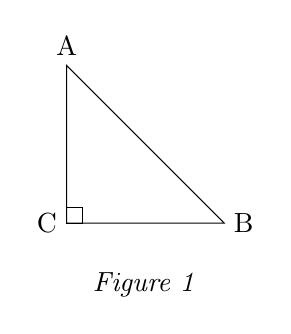
\begin{tikzpicture}
   		\coordinate (A) at (0,2);
   		\coordinate (C) at (0,0);
   		\coordinate (B) at (2,0);
   		
   		\draw (A)--(C)--(B)--cycle;
   		\draw (0,0) rectangle (0.2,0.2);
   		
   		\node [above] at (A) {A};
   		\node [left] at (C) {C};
   		\node [right] at (B) {B};
   		
   		\node [below] at (1,-0.5) {\textit{Figure 1}};
   	\end{tikzpicture}
   	\end{center}
   	
   	\solution
   	Triangle is a right-angled triangle at C and is isoceles.Because hypotenuse AB is the longest side, the two equal legs are AC and BC:
   	\begin{align*}
   		BC = AC = 4\text{ cm}
   	\end{align*}
   	
   	Applying the Pythagoras theorem in right-angled triangle ABC:
   	\begin{align*}
   		AB^2 &= AC^2 + BC^2 &\implies AB^2 &= 4^2 + 4^2 &\implies AB &= \sqrt{32} &\implies AB &= 4\sqrt{2}\text{ cm}
   	\end{align*}
   	
   	Therefore, the length of AB is:
   	\begin{align*}
   		AB = 4\sqrt{2}\text{ cm}
   	\end{align*}
   	
  
   	\item In Figure 2,DE $\parallel$ BC.Find the length of side AD,given that AE = 1·8 cm,BD = 7·2 cm and CE = 5·4 cm.
   	
\begin{center}
   	\begin{tikzpicture}
   		\coordinate (A) at (2.4,4);
   		\coordinate (C) at (0,0);
   		\coordinate (B) at (4,1);
   		\coordinate (D) at ($(A)!0.25!(B)$);
   		\coordinate (E) at ($(A)!0.25!(C)$); 
   		
   		\draw[thick] (A)--(C)--(B)--cycle;
   		\draw[thick] (D)--(E);
   		
   		\draw[->,thick] ($(D)!0.4!(E)$)--($(D)!0.55!(E)$);
   		\draw[->,thick] ($(B)!0.4!(C)$)--($(B)!0.55!(C)$);
   		
   		\node [above] at (A) {A};
   		\node [right] at (D) {D};
   		\node [left] at (E) {E};
   		\node [below left] at (B) {B};
   		\node [below right] at (C) {C};
   		
   		%Length labels
   		\node [left] at ($(B)!0.55!(D)$) {7.2 cm};
   		\node [right] at ($(A)!0.5!(E)$) {1.8 cm};
   		\node [right] at ($(E)!0.5!(C)$) {5.4 cm};
   		
   		\node [below] at (2.5,-0.55) {\textit{Figure 2}};
   	\end{tikzpicture}
   \end{center}
   
   \solution
   In triangle ABC, it is given that DE is parallel to BC. $DE \parallel BC$
   
   By the Basic Proportionality Theorem (Thales' Theorem):
   \begin{align*}
   	\frac{AD}{BD} &= \frac{AE}{CE}
   \end{align*}
   
   Substituting the given values[cite: 5]:
   \begin{align*}
   	\frac{AD}{7.2} &= \frac{1.8}{5.4} &\implies \frac{AD}{7.2} &= \frac{1}{3} &\implies AD &= \frac{7.2}{3} &\implies AD &= 2.4\text{ cm}
   \end{align*}
   
   Therefore, the length of side AD is:
   \begin{align*}
   	AD = 2.4\text{ cm}
   \end{align*}
   
   
   \item Find the nature of roots of the quadratic equation $2x^2 -4x + 3 = 0$.
   
   \solution
  We obtain[:
  \begin{align*}
  	a &= 2 &
  	b &= -4 &
  	c &= 3
  \end{align*}
  
  The discriminant is defined as:
  \begin{align*}
  	D &= b^2 - 4ac
  \end{align*}
  
  Substituting the values of a, b, and c:
  \begin{align*}
  	D &= (-4)^2 - 4(2)(3) 
  	= 16 - 24 
  	= -8
  \end{align*}
  
  Since the discriminant is less than zero:
  \begin{align*}
  	D < 0
  \end{align*}
  
  Therefore, the given quadratic equation has no real roots.
   NEED TO ADD GRAPH AND PYTHON CODE
  
	\item If HCF (336, 54) = 6, find LCM (336, 54).
	
	\solution
	Let the two given numbers be: $\text{a}=336$  $\text{b}=54$
	
	\begin{align*}
		\text{HCF}(a, b) = 6
	\end{align*}
	
	Using the property relating the HCF and LCM of two numbers:
	\begin{align*}
		\text{HCF}(a, b) \times \text{LCM}(a, b) &= a \times b
	\end{align*}
	
	Rearranging the equation to solve for the LCM:
	\begin{align*}
		\text{LCM}(a, b) &= \frac{a \times b}{\text{HCF}(a, b)}
	\end{align*}
	
	\begin{align*}
		\text{LCM}(336, 54) &= \frac{336 \times 54}{6} = 336 \times 9 = 3024
	\end{align*}
	
	Therefore, the value of the LCM is:
	\begin{align*}
		\text{LCM}(336, 54) = 3024
	\end{align*}
	
	
	\item Find the $21^{\text{st}}$ term of the A.P.$-4\frac{1}{2},\ -3,\ -1\frac{1}{2},\ \ldots$
	
	\solution
	The common difference d is:
	\begin{align*}
		d &= a_2 - a \\
		= -3 - \left(-\frac{9}{2}\right) 
		= -3 + \frac{9}{2} 
		= \frac{-6 + 9}{2} 
		= \frac{3}{2}
	\end{align*}
	
	The general formula for the n-th term of an arithmetic progression is:
	\begin{align*}
		a_n = a + (n - 1)d
	\end{align*}
	
	Substituting n = 21 to find the 21st term:
	\begin{align*}
		a_{21} &= -\frac{9}{2} + (21 - 1)\left(\frac{3}{2}\right) \\
		= -\frac{9}{2} + 20\left(\frac{3}{2}\right) 
		= -\frac{9}{2} + 30 
		= \frac{-9 + 60}{2} 
		= \frac{51}{2}
	\end{align*}
	
	Therefore, the 21st term of the A.P. is:
	\begin{align*}
		a_{21} = \frac{51}{2} \quad \left(\text{or } 25\frac{1}{2}\right)
	\end{align*}	
 
	\item For what value of $k$ will  have infinitely many solutions for the equations $2x+3y=7$ and $(k+2)x-3(1-k)y=5k+1$.
	
	\solution
	
	Form the augmented matrix for the linear network:
	\begin{align*}
		[\mathbf{A} \mid \mathbf{b}] = \left[\begin{array}{cc|c} 2 & 3 & 7 \\ k+2 & 3k-3 & 5k+1 \end{array}\right]
	\end{align*}
	
	Perform the elementary row operation:
	\begin{align*}
		R_2 \leftarrow 2R_2 - (k+2)R_1
	\end{align*}
	
	Evaluating the elements of the second row:
	\begin{align*}
		\text{First column: } & 2(k+2) - 2(k+2) = 0 \\
		\text{Second column: } & 2(3k-3) - 3(k+2) = 6k - 6 - 3k - 6 = 3k - 12 \\
		\text{Augmented column: } & 2(5k+1) - 7(k+2) = 10k + 2 - 7k - 14 = 3k - 12
	\end{align*}
	
	The matrix reduces to:
	\begin{align*}
		\left[\begin{array}{cc|c} 2 & 3 & 7 \\ 0 & 3k-12 & 3k-12 \end{array}\right]
	\end{align*}
	
	For the system to have infinitely many solutions, the second row must become a row of complete zeros (creating a free variable and ensuring consistency):
	\begin{align*}
		3k - 12 &= 0 \implies 3k = 12 \implies k = 4
	\end{align*}
	
	

	\item  Find the mode of the following frequency distribution:
	
	\begin{center}
		\begin{tabular}{|c|c|c|c|c|c|c|}
			\hline
			Class Interval & 25--30 & 30--35 & 35--40 &
			40--45 & 45--50 & 50--55\\
			\hline
			Frequency & 25 & 34 & 50 & 42 & 38 & 14\\
			\hline
		\end{tabular}
	\end{center}
	
	\solution
	The maximum frequency is 50, which lies in the class interval 35--40. Therefore, the modal class is 35--40[cite: 5].
	
	From the modal class:
	\begin{align*}
		\text{Lower limit, } l = 35 \\
		\text{Class size, } h = 40 - 35 = 5 \\
		\text{Frequency of modal class, } f_1 = 50 \\
		\text{Frequency of class preceding modal class, } f_0 = 34 \\
		\text{Frequency of class succeeding modal class, } f_2 = 42
	\end{align*}
	
	The formula for the mode of grouped data is:
	\begin{align*}
		\text{Mode} &= l + \left(\frac{f_1 - f_0}{2f_1 - f_0 - f_2}\right) \times h
	\end{align*}
	
	Substituting the values:
	\begin{align*}
		\text{Mode} &= 35 + \left(\frac{50 - 34}{2(50) - 34 - 42}\right) \times 5 \\
		&= 35 + \left(\frac{16}{24}\right) \times 5 \\
		&= 35 + \frac{10}{3} \\
		&= 38.33
	\end{align*}

	
	\item The larger of two supplementary angles exceeds the smaller by
	$18^\circ$. Find the angles.
	
	\solution
	Let the larger angle be x and the smaller angle be y.
	
	Since the two angles are supplementary, their sum is 180 degrees:
	\begin{align*}
		x + y = 180^\circ
	\end{align*}
	
	The larger angle exceeds the smaller by 18 degrees
	\begin{align*}
		x - y = 18^\circ
	\end{align*}
	
	Adding both equations:
	\begin{align*}
		(x + y) + (x - y) &= 180^\circ + 18^\circ \\
		2x &= 198^\circ \implies x = 99^\circ
	\end{align*}
	
	Substituting the value of x into the first equation:
	\begin{align*}
		99^\circ + y &= 180^\circ \implies y = 81^\circ
	\end{align*}
	
	Therefore, the two supplementary angles are:
	\begin{align*}
		x &= 99^\circ & y &= 81^\circ
	\end{align*}
	
	
	\item Sumit is 3 times as old as his son. Five years later, he shall be two and a half times as old as his son. How old is Sumit at present?
	
	\solution
	Let the present age of the son be: x \text{ years}
	
	Then, the present age of Sumit is: y = 3x
	
	Five years later:
	\begin{align*}
		\text{Son's age} &= x + 5 \\
		\text{Sumit's age} &= y + 5
	\end{align*}
	
	According to the given condition, Sumit will be two and a half times as old as his son:
	\begin{align*}
		y + 5 &= \frac{5}{2}(x + 5) \implies 2y + 10 & = 5x + 25
	\end{align*}
	
	Substituting y = 3x into the equation:
	\begin{align*}
		2(3x) + 10 &= 5x + 25 \\
		6x - 5x &= 25 - 10 \implies x = 15
	\end{align*}
	
	Now, finding Sumit's present age:
	\begin{align*}
		y &= 3x \\
		y &= 45
	\end{align*}
	
	
	\item  The probability of selecting a blue marble at random from a jar that contains only blue, black and green marbles is $\frac{1}{5}$. The probability of selecting a black marble at random from the same jar is $\frac{1}{4}$. If the jar contains 11 green marbles, find the total number of marbles in the jar.
	
	\solution
	Let the total number of marbles in the jar be n.
	
	Since the jar contains only blue, black, and green marbles, the sum of probabilities of all possible outcomes is equal to 1:
	\begin{align*}
		P(\text{blue}) + P(\text{black}) + P(\text{green}) &= 1
	\end{align*}
	
	
	Substituting these values to determine the probability of selecting a green marble:
	\begin{align*}
		\frac{1}{5} + \frac{1}{4} + P(\text{green}) &= 1 \\
		\frac{9}{20} + P(\text{green}) &= 1 \implies
		P(\text{green}) = \frac{11}{20}
	\end{align*}
	
	The probability of selecting a green marble is also given by the ratio of green marbles to total marbles:
	\begin{align*}
		P(\text{green}) &= \frac{\text{Number of green marbles}}{\text{Total number of marbles}} \implies 
		\frac{11}{20} = \frac{11}{n} \implies
		n = 20
	\end{align*}
	
	
	
	
	
	\item  Find a relation between $x$ and $y$ if the points
	$A(x,y)$, $B(-4,6)$ and $C(-2,3)$ are collinear.
	
	\solution
	Construct the displacement vectors with point A as the reference origin:
	\begin{align*}
		\mathbf{v}_1 &= \vec{AB} = \begin{bmatrix} -4 - x \\ 6 - y \end{bmatrix} \\
		\mathbf{v}_2 &= \vec{BC} = \begin{bmatrix} -2 - (-4) \\ 3 - 6 \end{bmatrix} = \begin{bmatrix} 2 \\ -3 \end{bmatrix}
	\end{align*}
	
	For collinearity, the vectors must be linearly dependent, meaning the column matrix formed by them has a rank of 1 and its determinant is zero:
	\begin{align*}
		\det \begin{bmatrix} \mathbf{v}_1 & \mathbf{v}_2 \end{bmatrix} &= 0 \\
		\det \begin{bmatrix} -4 - x & 2 \\ 6 - y & -3 \end{bmatrix} &= 0 \\
		(-4 - x)(-3) - (2)(6 - y) &= 0 \implies 3x + 2y = 0
	\end{align*}
	
	\item Find the area of a triangle whose vertices are
	$(1,-1)$, $(-4,6)$ and $(-3,-5)$.
	
	\solution
	Taking the first vertex as the origin, form two displacement edge vectors:
	\begin{align*}
		\mathbf{u} &= \vec{AB} = \begin{bmatrix} -4 - 1 \\ 6 - (-1) \end{bmatrix} = \begin{bmatrix} -5 \\ 7 \end{bmatrix} \\
		\mathbf{v} &= \vec{AC} = \begin{bmatrix} -3 - 1 \\ -5 - (-1) \end{bmatrix} = \begin{bmatrix} -4 \\ -4 \end{bmatrix}
	\end{align*}
	
	The area corresponds to half the absolute value of the 2x2 determinant formed by these column vectors:
	\begin{align*}
		\text{Area} &= \frac{1}{2} \left| \det \begin{bmatrix} \mathbf{u} & \mathbf{v} \end{bmatrix} \right| \\
		&= \frac{1}{2} \left| \det \begin{bmatrix} -5 & -4 \\ 7 & -4 \end{bmatrix} \right| \\
		&= \frac{1}{2} \left| 48 \right| = 24\text{ sq. units}
	\end{align*}
	

	\item  Write the smallest number which is divisible by both 306 and 657.
	
	\solution
	Compute the HCF of the two numbers using Euclid's division lemma:
	\begin{align*}
		657 &= 306 \times 2 + 45 \\
		306 &= 45 \times 6 + 36 \\
		45 &= 36 \times 1 + 9 \\
		36 &= 9 \times 4 + 0
	\end{align*}
	
	Since the remainder is 0, the HCF is:
	\begin{align*}
		\text{HCF}(306, 657) = 9
	\end{align*}
	
	Using the property relating the HCF and LCM of two numbers:
	\begin{align*}
		\text{LCM}(a, b) &= \frac{a \times b}{\text{HCF}(a, b)} \\
		\text{LCM}(306, 657) &= \frac{306 \times 657}{9} \\
		&= 34 \times 657 \\
		&= 22338
	\end{align*}

	\item  Point $A$ lies on the line segment $XY$ joining
	$X(6,-6)$ and $Y(-4,-1)$ in such a way that $\frac{XA}{XY}=\frac{2}{5}.$ If point $A$ also lies on the line $3x+k(y+1)=0$.find the value of $k$.
	
	\solution
	Point A lies on the line segment XY such that[cite: 6]:
	\begin{align*}
		\frac{XA}{XY} &= \frac{2}{5} \\
		\frac{XA}{XA + AY} &= \frac{2}{5} \\
		5XA &= 2(XA + AY) \\
		3XA &= 2AY \\
		\frac{XA}{AY} &= \frac{2}{3}
	\end{align*}
	
	Thus, point A divides the segment joining X(6, -6) and Y(-4, -1) internally in the ratio:
	\begin{align*}
		m : n = 2 : 3
	\end{align*}
	
	Using the section formula for coordinates of point A:
	\begin{align*}
		x &= \frac{m x_2 + n x_1}{m + n} \\
		&= \frac{2(-4) + 3(6)}{2 + 3} \\
		&= \frac{10}{5} = 2
	\end{align*}
	
	\begin{align*}
		y &= \frac{m y_2 + n y_1}{m + n} \\
		&= \frac{2(-1) + 3(-6)}{2 + 3} \\
		&= \frac{-20}{5} = -4
	\end{align*}
	
	Therefore, the coordinates of point A are:
	\begin{align*}
		A(2, -4)
	\end{align*}
	
	Since point A(2, -4) lies on the given line:
	\begin{align*}
		3x + k(y + 1) &= 0 \\
		3(2) + k(-4 + 1) &= 0 \\
		6 - 3k &= 0 \implies k = 2
	\end{align*}
	
	
	\item  Solve for $x$: $x^2+5x-(a^2+a-6)=0$.
	
	\solution
    The equation with the standard quadratic form $Ax^2 + Bx + C = 0$
	\begin{align*}
		A &= 1 & 	B &= 5  & 	C &= -(a^2 + a - 6)
	\end{align*}
	
	The discriminant $D$ is:
	\begin{align*}
		D &= B^2 - 4AC \\
		&= 5^2 - 4(1)\left[-(a^2 + a - 6)\right] \\
		&= 4a^2 + 4a + 1 = (2a + 1)^2
	\end{align*}
	
	Using the quadratic formula:
	\begin{align*}
		x &= \frac{-B \pm \sqrt{D}}{2A} \\
		&= \frac{-5 \pm \sqrt{(2a + 1)^2}}{2(1)} \\
		&= \frac{-5 \pm (2a + 1)}{2}
	\end{align*}
	
	Taking the positive sign:
	\begin{align*}
		x &= \frac{-5 + (2a + 1)}{2} \\
		&= \frac{2a - 4}{2} = a - 2
	\end{align*}
	
	Taking the negative sign:
	\begin{align*}
		x &= \frac{-5 - (2a + 1)}{2} \\
		&= \frac{-2a - 6}{2} = -(a + 3)
	\end{align*}
	
	Therefore, the values of $x$ are:
	\begin{align*}
		x = a - 2 \quad \text{(or)} \quad x = -(a + 3)
	\end{align*}
	
		
	\item  Find $A$ and $B$ if $\sin(A+2B)=\frac{\sqrt{3}}{2}$ and $\cos(A+4B)=0,$ where $A$ and $B$ are acute angles.
	
	\solution
	where $A$ and $B$ are acute angles[cite: 1]. \textit{(Note: Corrected from $\frac{3}{2}$ to $\frac{\sqrt{3}}{2}$ since the range of the sine function for real angles is $[-1, 1]$)}[cite: 1].
	
	\solution

	Since $\sin(60^\circ) = \frac{\sqrt{3}}{2}$ and the angles are acute:
	\begin{align*}
		A + 2B &= 60^\circ
	\end{align*}
	
	Since $\cos(90^\circ) = 0$:
	\begin{align*}
		A + 4B &= 90^\circ
	\end{align*}
	
	Writing the system of linear equations in matrix form $\mathbf{M}\mathbf{x} = \mathbf{b}$:
	\begin{align*}
		\begin{bmatrix} 1 & 2 \\ 1 & 4 \end{bmatrix} \begin{bmatrix} A \\ B \end{bmatrix} = \begin{bmatrix} 60^\circ \\ 90^\circ \end{bmatrix}
	\end{align*}
	
	The determinant of the system matrix $\mathbf{M}$ is:
	\begin{align*}
		\det(\mathbf{M}) = (1)(4) - (2)(1) = 2
	\end{align*}
	
	The inverse matrix $\mathbf{M}^{-1}$ is:
	\begin{align*}
		\mathbf{M}^{-1} = \frac{1}{2} \begin{bmatrix} 4 & -2 \\ -1 & 1 \end{bmatrix}
	\end{align*}
	
	Solving for state vector $\mathbf{x}$:
	\begin{align*}
		\begin{bmatrix} A \\ B \end{bmatrix} &= \frac{1}{2} \begin{bmatrix} 4 & -2 \\ -1 & 1 \end{bmatrix} \begin{bmatrix} 60^\circ \\ 90^\circ \end{bmatrix} \\
		&= \frac{1}{2} \begin{bmatrix} 4(60^\circ) - 2(90^\circ) \\ -1(60^\circ) + 1(90^\circ) \end{bmatrix} = \frac{1}{2} \begin{bmatrix} 60^\circ \\ 30^\circ \end{bmatrix} = \begin{bmatrix} 30^\circ \\ 15^\circ \end{bmatrix}
	\end{align*}
	
	Therefore, the values of $A$ and $B$ are:
	\begin{align*}
		A &= 30^\circ &	B = 15^\circ
	\end{align*}
	
	\item  Prove that $2+5\sqrt{3}$ is an irrational number, given that $\sqrt{3}$ is an irrational number.
	
	\solution
	Assume to the contrary that $2 + 5\sqrt{3}$ is a rational number.
	
	Then, it can be expressed in the form $\frac{a}{b}$, where $a$ and $b$ are co-prime integers and $b \neq 0$:
	\begin{align*}
		2 + 5\sqrt{3} &= \frac{a}{b}
	\end{align*}
	
	Rearranging the terms:
	\begin{align*}
		5\sqrt{3} &= \frac{a}{b} - 2 \\
		5\sqrt{3} &= \frac{a - 2b}{b} \\
		\sqrt{3} &= \frac{a - 2b}{5b}
	\end{align*}
	
	Since $a$ and $b$ are integers, $a - 2b$ and $5b$ are also integers ($5b \neq 0$). Thus, the right-hand side represents a rational number:
	\begin{align*}
		\frac{a - 2b}{5b} \in \mathbb{Q}
	\end{align*}
	
	This implies:
	\begin{align*}
		\sqrt{3} \in \mathbb{Q}
	\end{align*}
	
	This contradicts the given fact that $\sqrt{3}$ is an irrational number[cite: 1].
	
	Therefore, our assumption that $2 + 5\sqrt{3}$ is rational is false, and $2 + 5\sqrt{3}$ is an irrational number.
	
	\item Using Euclid's Algorithm, find the HCF of 2048 and 960.
	
	\solution
	The Euclidean algorithm corresponds to applying elementary unimodular shear matrices to reduce an integer state vector to its principal generator in a 1D lattice:
	\begin{align*}
		\mathbf{v}_0 = \begin{bmatrix} 2048 \\ 960 \end{bmatrix}
	\end{align*}
	
	Applying the first shear transformation $\mathbf{E}_1 = \begin{bmatrix} 1 & -2 \\ 0 & 1 \end{bmatrix}$:
	\begin{align*}
		\mathbf{v}_1 &= \mathbf{E}_1 \mathbf{v}_0 \\
		&= \begin{bmatrix} 1 & -2 \\ 0 & 1 \end{bmatrix} \begin{bmatrix} 2048 \\ 960 \end{bmatrix} 
		= \begin{bmatrix} 2048 - 2(960) \\ 960 \end{bmatrix} 
		= \begin{bmatrix} 128 \\ 960 \end{bmatrix}
	\end{align*}
	
	Applying the second shear transformation $\mathbf{E}_2 = \begin{bmatrix} 1 & 0 \\ -7 & 1 \end{bmatrix}$:
	\begin{align*}
		\mathbf{v}_2 &= \mathbf{E}_2 \mathbf{v}_1 \\
		&= \begin{bmatrix} 1 & 0 \\ -7 & 1 \end{bmatrix} \begin{bmatrix} 128 \\ 960 \end{bmatrix} 
		= \begin{bmatrix} 128 \\ 960 - 7(128) \end{bmatrix} 
		= \begin{bmatrix} 128 \\ 64 \end{bmatrix}
	\end{align*}
	
	Applying the third shear transformation $\mathbf{E}_3 = \begin{bmatrix} 1 & -2 \\ 0 & 1 \end{bmatrix}$:
	\begin{align*}
		\mathbf{v}_3 &= \mathbf{E}_3 \mathbf{v}_2 \\
		&= \begin{bmatrix} 1 & -2 \\ 0 & 1 \end{bmatrix} \begin{bmatrix} 128 \\ 64 \end{bmatrix} 
		= \begin{bmatrix} 128 - 2(64) \\ 64 \end{bmatrix} 
		= \begin{bmatrix} 0 \\ 64 \end{bmatrix}
	\end{align*}
	
	The non-zero invariant entry of the completely reduced state vector yields the greatest common divisor:
	\begin{align*}
		\gcd(2048, 960) = 64
	\end{align*}
 
 
 
	
	
	\item  Two right triangles $ABC$ and $DBC$ are drawn on the same hypotenuse $BC$ and on the same side of $BC$. If $AC$ and $BD$ intersect at $P$, prove that $AP\times PC=BP\times DP$.
 
	
	\begin{center}
		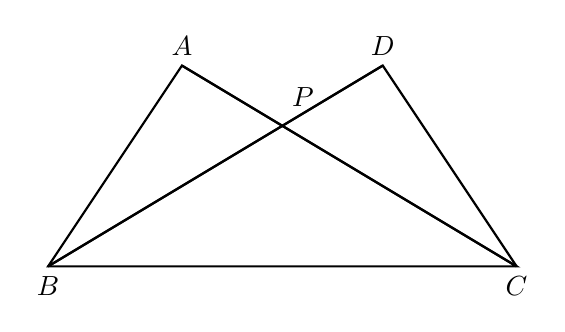
\begin{tikzpicture}[scale=0.85]
			\coordinate (B) at (0,0);
			\coordinate (C) at (7,0);
			\coordinate (A) at (2,3);
			\coordinate (D) at (5,3);
			\coordinate (P) at (3.5,2.25);
			
			\draw[thick] (B)--(A)--(C)--cycle;
			\draw[thick] (B)--(D)--(C);
			\draw[thick] (A)--(C);
			\draw[thick] (B)--(D);
			
			\node[above] at (A) {$A$};
			\node[above] at (D) {$D$};
			\node[below] at (B) {$B$};
			\node[below] at (C) {$C$};
			\node[above right] at (P) {$P$};
		\end{tikzpicture}
	\end{center}
	
	\solution
	In right triangles $ABC$ and $DBC$, both are right-angled on the same hypotenuse $BC$:
	\begin{align*}
		\angle BAC &= 90^\circ & \angle BDC &= 90^\circ
	\end{align*}
	
	Since hypotenuse $BC$ subtends equal angles of $90^\circ$ at vertices $A$ and $D$ on the same side, the four points $A$, $B$, $C$, and $D$ are concyclic, lying on a circle with diameter $BC$[cite: 1].
	
	For the chord $AD$, the angles subtended in the same segment of the circle are equal:
	\begin{align*}
		\angle ABD &= \angle ACD & \angle PBA &= \angle PCD
	\end{align*}
	
	Now, compare $\triangle PAB$ and $\triangle PDC$:
	\begin{align*}
		\angle APB &= \angle DPC \quad (\text{vertically opposite angles}) \\
		\angle PBA &= \angle PCD \quad (\text{angles in the same segment})
	\end{align*}
	
	By the AA (Angle-Angle) similarity criterion:
	\begin{align*}
		\triangle PAB \sim \triangle PDC
	\end{align*}
	
	Since the ratio of corresponding sides of similar triangles is equal:
	\begin{align*}
		\frac{AP}{DP} &= \frac{BP}{PC} \implies 	AP \times PC = BP \times DP
	\end{align*}
	
 
	
	
	
 
	\item Diagonals of a trapezium $PQRS$ intersect each other at the point $O$,
	$PQ\parallel RS$ and $PQ=3RS$. Find the ratio of the areas of triangles $POQ$ and $ROS$.
	
	\begin{center}
		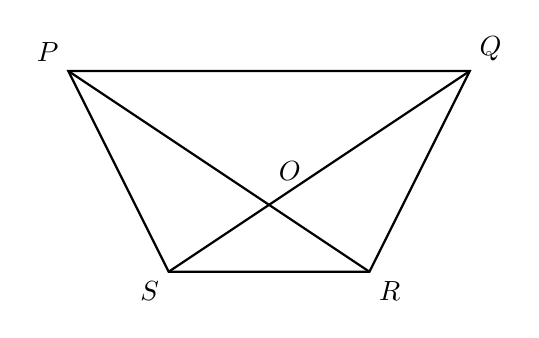
\begin{tikzpicture}[scale=0.85]
			\coordinate (P) at (0,3);
			\coordinate (Q) at (6,3);
			\coordinate (R) at (4.5,0);
			\coordinate (S) at (1.5,0);
			\coordinate (O) at (3,1.5);
			
			\draw[thick] (P)--(Q)--(R)--(S)--cycle;
			\draw[thick] (P)--(R);
			\draw[thick] (Q)--(S);
			
			\node[above left] at (P) {$P$};
			\node[above right] at (Q) {$Q$};
			\node[below right] at (R) {$R$};
			\node[below left] at (S) {$S$};
			\node[right] at (O) {$O$};
		\end{tikzpicture}
	\end{center}
	
	\solution
	In trapezium $PQRS$, it is given that $PQ \parallel RS$[cite: 1].
	
	In $\triangle POQ$ and $\triangle ROS$:
	\begin{align*}
		\angle POQ &= \angle ROS \quad (\text{vertically opposite angles}) \\
		\angle OPQ &= \angle ORS \quad (\text{alternate interior angles, as } PQ \parallel RS) \\
		\angle OQP &= \angle OSR \quad (\text{alternate interior angles, as } PQ \parallel RS)
	\end{align*}
	
	Therefore, by the AAA similarity criterion:
	\begin{align*}
		\triangle POQ \sim \triangle ROS
	\end{align*}
	
	The ratio of the areas of two similar triangles is equal to the square of the ratio of their corresponding sides:
	\begin{align*}
		\frac{\text{Area}(\triangle POQ)}{\text{Area}(\triangle ROS)} &= \left(\frac{PQ}{RS}\right)^2
	\end{align*}
	
	Given that $PQ = 3RS$ :
	\begin{align*}
		\frac{\text{Area}(\triangle POQ)}{\text{Area}(\triangle ROS)} &= \left(\frac{3RS}{RS}\right)^2  = (3)^2 = \frac{9}{1}
	\end{align*}
	
	
	
	\item  In Figure 3, $PQ$ and $RS$ are two parallel tangents to a circle with centre $O$ and another tangent $AB$ with point of contact $C$ intersects $PQ$ at $A$ and $RS$ at $B$. Prove that $	\angle AOB=90^\circ$.
	
	\begin{center}
		\begin{tikzpicture}[>=Stealth, line cap=round, line join=round, thick]
			
		
			\def\r{2.0}          % Radius of the circle
			\def\alphaAng{55}    % Angle DOA (degrees)
			
		
			\coordinate (O) at (0, 0);
			\coordinate (D) at (0, \r);
			\coordinate (E) at (0, -\r);
			
			
			\pgfmathsetmacro{\xA}{\r * tan(\alphaAng)}
			\pgfmathsetmacro{\xB}{\r * tan(90 - \alphaAng)}
			\pgfmathsetmacro{\angC}{90 - 2*\alphaAng}
			
			\coordinate (A) at (\xA, \r);
			\coordinate (B) at (\xB, -\r);
			\coordinate (C) at (\angC:\r);
			
			\draw (O) circle (\r);
			
			\draw [<->] (-2.5, \r) -- (4.2, \r);
			\draw [<->] (-2.5, -\r) -- (4.2, -\r);
		 
			\draw (A) -- (B);
			\draw (O) -- (A);
			\draw (O) -- (B);
			
		 
			\fill (O) circle (1.8pt) node[left=1pt] {$O$};
			\fill (D) circle (1.8pt) node[above=2pt] {$D$};
			\fill (E) circle (1.8pt) node[below=2pt] {$E$};
			\fill (A) circle (1.8pt) node[above=2pt] {$A$};
			\fill (B) circle (1.8pt) node[below=2pt] {$B$};
			\fill (C) circle (1.8pt) node[right=2pt] {$C$};
			
		 
			\node[above] at (-2.0, \r) {$P$};
			\node[above] at (3.6, \r) {$Q$};
			\node[below] at (-2.0, -\r) {$R$};
			\node[below] at (3.6, -\r) {$S$};
			
			% --- Figure Caption ---
			\node[below=8pt] at (0.6, -\r) {\textit{Figure 3}};
			
		\end{tikzpicture}
	\end{center}
	
	\solution
	Let $O$ be the origin $(0,0)$. With tangent hyperplanes $y = r$ ($PQ$) and $y = -r$ ($RS$), parameterize contact point $C$ on circle $\|\mathbf{x}\| = r$ by $\theta \in (-\pi/2, \pi/2)$:
	\begin{align*}
		\mathbf{r}_C = \begin{bmatrix} r\cos\theta \\ r\sin\theta \end{bmatrix}
	\end{align*}
	
	The tangent hyperplane normal at $C$ is $\mathbf{\hat{n}} = [\cos\theta, \, \sin\theta]^T$, yielding line equation $x\cos\theta + y\sin\theta = r$. Intersecting with boundaries $y = \pm r$:
	\begin{align*}
		\mathbf{r}_A = \begin{bmatrix} r\frac{1-\sin\theta}{\cos\theta} \\ r \end{bmatrix}, \quad \mathbf{r}_B = \begin{bmatrix} r\frac{1+\sin\theta}{\cos\theta} \\ -r \end{bmatrix}
	\end{align*}
	
	Evaluating the inner product:
	\begin{align*}
		\langle \mathbf{r}_A, \mathbf{r}_B \rangle &= r^2 \left(\frac{1 - \sin^2\theta}{\cos^2\theta}\right) - r^2 = r^2(1) - r^2 = 0
	\end{align*}
	
	Since $\langle \mathbf{r}_A, \mathbf{r}_B \rangle = 0$, position vectors $\mathbf{r}_A \perp \mathbf{r}_B \implies \angle AOB = 90^\circ$.
	
	
	\item In Figure 4, a square $OABC$ is inscribed in a quadrant $OPBQ$. If $OA=15$ cm, find the area of the shaded region. (Use $\pi=3.14$.)
	
	\begin{center}
		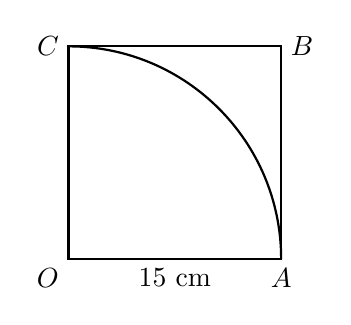
\begin{tikzpicture}[scale=0.18]
			\coordinate (O) at (0,0);
			\coordinate (A) at (15,0);
			\coordinate (B) at (15,15);
			\coordinate (C) at (0,15);
			
			\fill[gray!30] (O)--(15,0) arc (0:90:15)--cycle;
			\fill[white] (O)--(A)--(B)--(C)--cycle;
			
			\draw[thick] (O)--(15,0);
			\draw[thick] (O)--(0,15);
			\draw[thick] (15,0) arc (0:90:15);
			\draw[thick] (O)--(A)--(B)--(C)--cycle;
			
			\node[below left] at (O) {$O$};
			\node[below] at (A) {$A$};
			\node[right] at (B) {$B$};
			\node[left] at (C) {$C$};
			\node[below] at (7.5,0) {$15$ cm};
		\end{tikzpicture}
	\end{center}
	
	\solution
	Let the side of the square $OABC$ be:
	\begin{align*}
		s = OA = AB = 15\text{ cm}
	\end{align*}
	
	In $\triangle OAB$, $\angle OAB = 90^\circ$. Diagonal $OB$ forms the radius $r$ of the circular quadrant $OPBQ$. Applying the Pythagoras theorem in right-angled triangle $OAB$:
	\begin{align*}
		OB^2 &= OA^2 + AB^2 \\
		OB^2 &= 15^2 + 15^2 \implies
		OB = \sqrt{450} = 15\sqrt{2}\text{ cm}
	\end{align*}
	
	Thus, the radius of the quadrant is:
	\begin{align*}
		r = 15\sqrt{2}\text{ cm}
	\end{align*}
	
	The area of quadrant $OPBQ$ is:
	\begin{align*}
		\text{Area of quadrant} &= \frac{1}{4}\pi r^2 = \frac{1}{4} \times 3.14 \times (15\sqrt{2})^2 
		= \frac{1413}{4} = 353.25\text{ cm}^2
	\end{align*}
	
	The area of square $OABC$ is:
	\begin{align*}
		\text{Area of square} &= s^2 = 15^2 = 225\text{ cm}^2
	\end{align*}
	
	The area of the shaded region is given by:
	\begin{align*}
		\text{Area of shaded region} &= \text{Area of quadrant} - \text{Area of square} \\
		&= 353.25 - 225 = 128.25\text{ cm}^2
	\end{align*}
	
	
 
	\item In Figure 5, $ABCD$ is a square with side $2\sqrt{2}$ cm and inscribed in a circle. Find the area of the shaded region. (Use $\pi=3.14$.)
	
	\begin{center}
		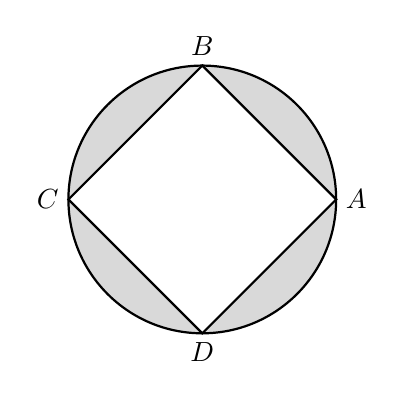
\begin{tikzpicture}[scale=0.85]
			\coordinate (O) at (0,0);
			\coordinate (A) at (2,0);
			\coordinate (B) at (0,2);
			\coordinate (C) at (-2,0);
			\coordinate (D) at (0,-2);
			
			\fill[gray!30] (O) circle (2);
			\fill[white] (A)--(B)--(C)--(D)--cycle;
			
			\draw[thick] (O) circle (2);
			\draw[thick] (A)--(B)--(C)--(D)--cycle;
			
			\node[right] at (A) {$A$};
			\node[above] at (B) {$B$};
			\node[left] at (C) {$C$};
			\node[below] at (D) {$D$};
		\end{tikzpicture}
	\end{center}
	
	\solution
	Let the side of the inscribed square $ABCD$ be[cite: 2]:
	\begin{align*}
		a = 2\sqrt{2}\text{ cm}
	\end{align*}
	
	Since each interior angle of a square is $90^\circ$, diagonal $AC$ subtends $90^\circ$ at the circle's circumference, meaning $AC$ is the diameter of the circumscribing circle:
	\begin{align*}
		AC^2 &= AB^2 + BC^2 \\
		AC^2 &= (2\sqrt{2})^2 + (2\sqrt{2})^2 \implies	AC = \sqrt{16} = 4\text{ cm}
	\end{align*}
	
	The radius $r$ of the circle is:
	\begin{align*}
		r = \frac{AC}{2} = \frac{4}{2} = 2\text{ cm}
	\end{align*}
	
	The area of the circumscribed circle is:
	\begin{align*}
		\text{Area of circle} &= \pi r^2 = 3.14 \times 2^2 = 3.14 \times 4 = 12.56\text{ cm}^2
	\end{align*}
	
	The area of the inscribed square is:
	\begin{align*}
		\text{Area of square} &= a^2 = (2\sqrt{2})^2 = 8\text{ cm}^2
	\end{align*}
	
	The area of the shaded region is:
	\begin{align*}
		\text{Area of shaded region} &= \text{Area of circle} - \text{Area of square} \\
		&= 12.56 - 8 = 4.56\text{ cm}^2
	\end{align*}
	
	
	\item A solid is in the form of a cylinder with hemispherical ends. The total height of the solid is 20 cm and the diameter of the cylinder is 7 cm. Find the total volume of the solid. (Use $\pi=\frac{22}{7}$.)
	
	\begin{center}
		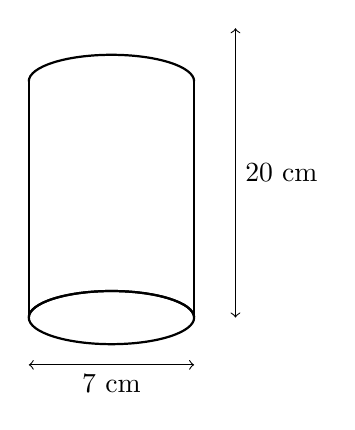
\begin{tikzpicture}[scale=0.75]
			\draw[thick] (0,0) arc (180:360:1.4 and 0.45);
			\draw[thick] (0,0) arc (180:0:1.4 and 0.45);
			\draw[thick] (0,0)--(0,4);
			\draw[thick] (2.8,0)--(2.8,4);
			\draw[thick] (0,4) arc (180:0:1.4 and 0.45);
			\draw[thick] (0,0) arc (180:0:1.4 and 0.45);
			
			\draw[<->] (3.5,0)--(3.5,4.9);
			\node[right] at (3.5,2.45) {20 cm};
			\draw[<->] (0,-0.8)--(2.8,-0.8);
			\node[below] at (1.4,-0.8) {7 cm};
		\end{tikzpicture}
	\end{center}
	
	\solution
	The solid comprises a central right circular cylinder capped by two identical hemispherical ends.
	
	From the given dimensions:
	\begin{align*}
		\text{Diameter, } d &= 7\text{ cm} \implies \text{Radius, } r = \frac{7}{2}\text{ cm} \\
		\text{Total height, } H &= 20\text{ cm}
	\end{align*}
	
	The height of the cylindrical portion $h$ is obtained by subtracting the radii of both hemispherical ends:
	\begin{align*}
		h &= H - 2r = 20 - 2\left(\frac{7}{2}\right) = 20 - 7 = 13\text{ cm}
	\end{align*}
	
	The volume of the cylindrical portion is:
	\begin{align*}
		V_{\text{cylinder}} &= \pi r^2 h \\
		&= \frac{22}{7} \times \left(\frac{7}{2}\right)^2 \times 13 
		= \frac{22}{7} \times \frac{49}{4} \times 13 
		= \frac{11 \times 7 \times 13}{2} = \frac{1001}{2} = 500.5\text{ cm}^3
	\end{align*}
	
	The two hemispherical ends combine to form a complete sphere of radius $r$:
	\begin{align*}
		V_{\text{ends}} &= 2 \times \left(\frac{2}{3}\pi r^3\right) = \frac{4}{3}\pi r^3 \\
		&= \frac{4}{3} \times \frac{22}{7} \times \left(\frac{7}{2}\right)^3 
		= \frac{4}{3} \times \frac{22}{7} \times \frac{343}{8} 
		= \frac{11 \times 49}{3} = \frac{539}{3} \approx 179.67\text{ cm}^3
	\end{align*}
	
	Summing the component volumes:
	\begin{align*}
		V_{\text{total}} &= V_{\text{cylinder}} + V_{\text{ends}} \\
		&= \frac{1001}{2} + \frac{539}{3} 
		= \frac{3003 + 1078}{6} 
		= \frac{4081}{6} = 680\frac{1}{6}\text{ cm}^3 \approx 680.17\text{ cm}^3
	\end{align*}
	
	
	\item The marks obtained by 100 students in an examination are given below:
	
	\begin{center}
		\begin{tabular}{|l|c|c|c|c|c|c|c|c|}
			\hline
			Marks & 30--35 & 35--40 & 40--45 & 45--50 &
			50--55 & 55--60 & 60--65\\
			\hline
			Number of Students & 14 & 16 & 28 & 23 & 18 & 8 & 3\\
			\hline
		\end{tabular}
	\end{center}
	Find the mean marks of the students.
	
	\solution
	
	\begin{center}
		\begin{tabular}{|c|c|c|}
			\hline
			\textbf{Marks} & \textbf{Class Mark ($x_i$)} & \textbf{Frequency ($f_i$)} \\
			\hline
			30--35 & 32.5 & 14 \\
			35--40 & 37.5 & 16 \\
			40--45 & 42.5 & 28 \\
			50--55 & 52.5 & 18 \\
			55--60 & 57.5 & 8  \\
			60--65 & 62.5 & 3  \\
			\hline
			\textbf{Total} & & $\sum f_i = 110$ \\
			\hline
		\end{tabular}
	\end{center}
	
	\begin{align*}
		\sum f_i x_i &= 14(32.5) + 16(37.5) + 28(42.5) + 23(47.5) + 18(52.5) + 8(57.5) + 3(62.5) \\
		&= 455 + 600 + 1190 + 1092.5 + 945 + 460 + 187.5 = 4930
	\end{align*}
	
	\begin{align*}
		\bar{x} &= \frac{\sum f_i x_i}{\sum f_i} = \frac{4930}{110} = \frac{493}{11} \approx 44.82
	\end{align*}
	

	\item For what value of $k$ is the polynomial $f(x)=3x^4-9x^3+x^2+15x+k$ completely divisible by $3x^2-5$?
	
	\solution
	Work in the quotient ring $\mathbb{R}[x] / \langle 3x^2 - 5 \rangle$, where the divisor induces the reduction relation:
	\begin{align*}
		3x^2 - 5 \equiv 0 \implies x^2 \equiv \frac{5}{3}
	\end{align*}
	
	Higher powers of the state variable $x$ reduce recursively:
	\begin{align*}
		x^3 &= x \cdot x^2 \equiv \frac{5}{3}x & x^4 &= (x^2)^2 \equiv \left(\frac{5}{3}\right)^2 = \frac{25}{9}
	\end{align*}
	
	Projecting $f(x)$ onto the 1st-degree polynomial subspace modulo $(3x^2 - 5)$:
	\begin{align*}
		f(x) &\equiv 3\left(\frac{25}{9}\right) - 9\left(\frac{5}{3}x\right) + \left(\frac{5}{3}\right) + 15x + k \pmod{3x^2 - 5} \\
		&\equiv \frac{25}{3} - 15x + \frac{5}{3} + 15x + k \equiv 10 + k
	\end{align*}
	
	Setting the residue projection to zero:
	\begin{align*}
		10 + k = 0 \implies k = -10
	\end{align*}
	
	
	\item Find the zeroes of the quadratic polynomial $7y^2-\frac{11}{3}y-\frac{2}{3}$ and verify the relationship between the zeroes and the coefficients.
	
	\solution
	Comparing $p(y) = 7y^2 - \frac{11}{3}y - \frac{2}{3}$ with standard quadratic form $a y^2 + b y + c$:
	\begin{align*}
		a = 7, \quad b = -\frac{11}{3}, \quad c = -\frac{2}{3}
	\end{align*}
	
	 Sum of zeroes:
	\begin{align*}
		\alpha + \beta &= \frac{2}{3} + \left(-\frac{1}{7}\right) = \frac{14 - 3}{21} = \frac{11}{21} = -\frac{b}{a}
	\end{align*}
	
	2. Product of zeroes:
	\begin{align*}
		\alpha \beta &= \left(\frac{2}{3}\right)\left(-\frac{1}{7}\right) = -\frac{2}{21} = 	\frac{c}{a} 
	\end{align*}
	
	
	
	\item Prove that the ratio of the areas of two similar
	triangles is equal to the ratio of the squares on their
	corresponding sides.
	
	
	\solution
	
    To Prove:
	\begin{align*}
		\frac{\text{ar}(\triangle ABC)}{\text{ar}(\triangle PQR)} = \left(\frac{AB}{PQ}\right)^2 = \left(\frac{BC}{QR}\right)^2 = \left(\frac{CA}{RP}\right)^2
	\end{align*}
	
	Proof:
	
	The area of a triangle is given by half the product of its base and corresponding altitude:
	\begin{align*}
		\text{ar}(\triangle ABC) &= \frac{1}{2} \times BC \times AM \\
		\text{ar}(\triangle PQR) &= \frac{1}{2} \times QR \times PN
	\end{align*}
	
	Taking the ratio of their areas:
	\begin{align*}
		\frac{\text{ar}(\triangle ABC)}{\text{ar}(\triangle PQR)} &= \frac{\frac{1}{2} \times BC \times AM}{\frac{1}{2} \times QR \times PN} = \left(\frac{BC}{QR}\right) \times \left(\frac{AM}{PN}\right)
	\end{align*}
	
	In $\triangle ABM$ and $\triangle PQN$:
	\begin{align*}
		\angle B &= \angle Q \quad (\text{corresponding angles of similar triangles, } \triangle ABC \sim \triangle PQR) \\
		\angle AMB &= \angle PNQ = 90^\circ \quad (\text{by construction})
	\end{align*}
	
	By the AA (Angle-Angle) similarity criterion:
	\begin{align*}
		\triangle ABM \sim \triangle PQN
	\end{align*}
	
	Since corresponding sides of similar triangles are in proportion:
	\begin{align*}
		\frac{AM}{PN} = \frac{AB}{PQ}
	\end{align*}
	
	Since $\triangle ABC \sim \triangle PQR$, their corresponding sides are proportional:
	\begin{align*}
		\frac{AB}{PQ} = \frac{BC}{QR} = \frac{CA}{RP}
	\end{align*}
	
	Substituting $\frac{AM}{PN} = \frac{BC}{QR}$ into the area ratio expression:
	\begin{align*}
		\frac{\text{ar}(\triangle ABC)}{\text{ar}(\triangle PQR)} &= \left(\frac{BC}{QR}\right) \times \left(\frac{BC}{QR}\right) = \left(\frac{BC}{QR}\right)^2
	\end{align*}
	
	Using the ratio equality of the corresponding sides:
	\begin{align*}
		\frac{\text{ar}(\triangle ABC)}{\text{ar}(\triangle PQR)} = \left(\frac{AB}{PQ}\right)^2 = \left(\frac{BC}{QR}\right)^2 = \left(\frac{CA}{RP}\right)^2
	\end{align*}
	
	
	
	
	
	\item  Two poles of equal heights are standing opposite
	to each other on either side of the road which is 80 m wide.
	From a point $P$ between them on the road, the angle of
	elevation of the top of a pole is $60^\circ$ and the angle of
	depression from the top of the other pole to point $P$ is
	$30^\circ$. Find the heights of the poles and the distance
	of the point $P$ from the poles.
	
	\begin{center}
		\begin{tikzpicture}[scale=0.8,>=Stealth]
			
			% Ground
			\draw[thick] (0,0)--(10,0);
			
			% Poles
			\draw[thick] (0,0)--(0,4);
			\draw[thick] (10,0)--(10,4);
			
			% Point P
			\coordinate (P) at (3,0);
			\fill (P) circle (2pt);
			\node[below] at (P) {$P$};
			
			% Tops
			\coordinate (T1) at (0,4);
			\coordinate (T2) at (10,4);
			
			% Lines of sight
			\draw[dashed] (P)--(T1);
			\draw[dashed] (P)--(T2);
			
			% Horizontal from top of right pole
			\draw[dotted] (10,4)--(3,4);
			
			% Labels
			\node[left] at (T1) {Top};
			\node[right] at (T2) {Top};
			
			\node[below] at (1.5,0) {$x$};
			\node[below] at (6.5,0) {$80-x$};
			
			\node[above] at (5,4) {Horizontal line};
			
			% Angles are illustrative
			\draw (P) ++(0.7,0) arc (0:53:0.7);
			\node at (4.0,0.45) {$60^\circ$};
			
			\draw (10,4) ++(-0.8,0) arc (180:225:0.8);
			\node at (8.9,3.45) {$30^\circ$};
			
			\node[below] at (5,-0.8) {Road width $=80$ m};
			
		\end{tikzpicture}
	\end{center}
	
	\solution
	From the two geometric projection constraints:
	\begin{align*}
		\sqrt{3}x - h &= 0 & x + \sqrt{3}h &= 80
	\end{align*}
	
	Formulating as a linear vector system $\mathbf{A}\mathbf{v} = \mathbf{b}$:
	\begin{align*}
		\begin{bmatrix} \sqrt{3} & -1 \\ 1 & \sqrt{3} \end{bmatrix} \begin{bmatrix} x \\ h \end{bmatrix} = \begin{bmatrix} 0 \\ 80 \end{bmatrix}
	\end{align*}
	
	\begin{align*}
		\mathbf{A} = 2 \begin{bmatrix} \cos(30^\circ) & -\sin(30^\circ) \\ \sin(30^\circ) & \cos(30^\circ) \end{bmatrix}
	\end{align*}
	
	The determinant is:
	\begin{align*}
		\det(\mathbf{A}) = (\sqrt{3})(\sqrt{3}) - (-1)(1) = 3 + 1 = 4
	\end{align*}
	
	The inverse matrix is:
	\begin{align*}
		\mathbf{A}^{-1} = \frac{1}{4} \begin{bmatrix} \sqrt{3} & 1 \\ -1 & \sqrt{3} \end{bmatrix}
	\end{align*}
	
	Solving for the state coordinates:
	\begin{align*}
		\begin{bmatrix} x \\ h \end{bmatrix} &= \frac{1}{4} \begin{bmatrix} \sqrt{3} & 1 \\ -1 & \sqrt{3} \end{bmatrix} \begin{bmatrix} 0 \\ 80 \end{bmatrix} 
		= \frac{1}{4} \begin{bmatrix} 80 \\ 80\sqrt{3} \end{bmatrix}
		= \begin{bmatrix} 20 \\ 20\sqrt{3} \end{bmatrix}
	\end{align*}
	
	Thus, $x = 20\text{ m}$ and $h = 20\sqrt{3}\text{ m}$.
	
	
	\item The total cost of a certain length of a piece of
	cloth is Rs.\ 200. If the piece was 5 m longer and each metre
	of cloth costs Rs.\ 2 less, the cost of the piece would have
	remained unchanged. How long is the piece and what is its
	original rate per metre?
	
	\solution
	
	\begin{align*}
		\text{Original rate} = \frac{200}{x}\text{ Rs./m}
	\end{align*}
	
	\begin{align*}
		\text{New length} &= (x + 5)\text{m} & \text{New rate} = \left(\frac{200}{x} - 2\right)\text{Rs./m}
	\end{align*}
	
	The total cost remains unchanged at Rs.\ 200:
	\begin{align*}
		(\text{New length}) \times (\text{New rate}) &= 200 \\
		(x + 5)\left(\frac{200}{x} - 2\right) &= 200
	\end{align*}
	
	Expanding the expression:
	\begin{align*}
		x\left(\frac{200}{x}\right) - 2x + 5\left(\frac{200}{x}\right) - 10 &= 200 \implies
		-2x + \frac{1000}{x} - 10 = 0\\
	 \implies -2x^2 - 10x + 1000 &= 0 \implies	x^2 + 5x - 500 = 0
	\end{align*}
	
	Factorising the quadratic equation:
	\begin{align*}
		x^2 + 25x - 20x - 500 &= 0 \implies (x - 20)(x + 25) = 0
	\end{align*}
	
	Equating each factor to zero:
	\begin{align*}
		x - 20 = 0 &\implies x = 20  & x + 25 = 0 \implies x = -25
	\end{align*}
	
	Since length cannot be negative, $x = 20\text{ m}$
	
	Evaluating the original rate per metre:
	\begin{align*}
		\text{Original rate} = \frac{200}{20} = 10\text{ Rs./m}
	\end{align*}
	
	
	
	\item Which term of the Arithmetic Progression $-7,\,-12,\,-17,\,-22,\,\ldots $will be $-82$? Is $-100$ any term of the A.P.? Give reason for your answer.
	
	\solution
	For the given Arithmetic Progression $-7, -12, -17, -22, \ldots$:
	\begin{align*}
		\text{First term, } a &= -7 & \text{Common difference, } d = -12 - (-7) = -5
	\end{align*}
	
	Let the $n^{\text{th}}$ term be $-82$:
	\begin{align*}
		a_n &= a + (n - 1)d \\
		-82 = -7 + (n - 1)(-5) \implies
		-75 = -5(n - 1) \\ 
		\implies n - 1 = \frac{-75}{-5} = 15 \implies
		n = 16
	\end{align*}
	
	Now, suppose $-100$ is the $m^{\text{th}}$ term of the progression:
	\begin{align*}
		a_m &= a + (m - 1)d \\
		-100 &= -7 + (m - 1)(-5) \\
		-100 + 7 &= -5(m - 1) \\
		m - 1 &= \frac{93}{5} = 18.6 \implies m = 19.6
	\end{align*}
	Since the term index $m$ must be a positive integer ($m \in \mathbb{Z}^+$), $-100$ cannot be a term of this A.P.
	
	
	\item How many terms of the Arithmetic Progression $45,\,39,\,33,\,\ldots$ must be taken so that their sum is 180? Explain the	double answer.
	
	\solution
	For the given Arithmetic Progression $45, 39, 33, \ldots$[cite: 3]:
	\begin{align*}
		\text{First term, } a &= 45 \\
		\text{Common difference, } d &= 39 - 45 = -6
	\end{align*}
	
	Let the sum of the first $n$ terms be $S_n = 180$:
	\begin{align*}
		S_n &= \frac{n}{2}\left[2a + (n - 1)d\right] \\
		180 &= \frac{n}{2}\left[2(45) + (n - 1)(-6)\right] \implies
		180 = n(48 - 3n) \implies
		180 = 48n - 3n^2
	\end{align*}
	
	Rearranging into standard quadratic form:
	\begin{align*}
		3n^2 - 48n + 180 &= 0 \implies
		n^2 - 16n + 60 = 0
	\end{align*}
	
	Factorising the quadratic equation:
	\begin{align*}
		n^2 - 10n - 6n + 60 &= 0 \implies
		(n - 6)(n - 10) = 0
	\end{align*}
	
	Equating each factor to zero:
	\begin{align*}
		n = 6 \quad \text{(or)} \quad n = 10
	\end{align*}
	
	Explanation of the double answer:
	
	The common difference is negative ($d = -6$), meaning the terms decrease and eventually become negative.
	
	Evaluating the terms from $n = 7$ to $n = 10$:
	\begin{align*}
		a_7 &= 45 + 6(-6) = 9 \\
		a_8 &= 45 + 7(-6) = 3 \\
		a_9 &= 45 + 8(-6) = -3 \\
		a_{10} &= 45 + 9(-6) = -9
	\end{align*}
	
	The sum of these additional four terms is:
	\begin{align*}
		a_7 + a_8 + a_9 + a_{10} &= 9 + 3 + (-3) + (-9) = 0
	\end{align*}
	
	Since the sum of the $7^{\text{th}}$, $8^{\text{th}}$, $9^{\text{th}}$, and $10^{\text{th}}$ terms is zero, adding them to the first 6 terms does not change the cumulative sum. Thus, both $n = 6$ and $n = 10$ give $S_n = 180$.
	
	
	\item Prove that
	\[
	\frac{\tan\theta}{1-\cot\theta}
	+
	\frac{\cot\theta}{1-\tan\theta}
	=
	1 + \sec \theta \csc \theta.
	\]
	
	\solution
	
	\begin{align*}
		\text{LHS} &= \frac{\tan\theta}{1 - \frac{1}{\tan\theta}} + \frac{\frac{1}{\tan\theta}}{1 - \tan\theta} = \frac{\tan^2\theta}{\tan\theta - 1} - \frac{1}{\tan\theta(\tan\theta - 1)}
	\end{align*}

	\begin{align*}
		\text{LHS} &= \frac{\tan^3\theta - 1}{\tan\theta(\tan\theta - 1)}
	\end{align*}
	
	Applying the algebraic cubic factorization $a^3 - b^3 = (a - b)(a^2 + ab + b^2)$:
	\begin{align*}
		\text{LHS} &= \frac{(\tan\theta - 1)(\tan^2\theta + \tan\theta + 1)}{\tan\theta(\tan\theta - 1)} \\
		&= \frac{\tan^2\theta + \tan\theta + 1}{\tan\theta} 
		= \tan\theta + 1 + \cot\theta
	\end{align*}
	
	\begin{align*}
		\text{LHS} &= 1 + \frac{\sin\theta}{\cos\theta} + \frac{\cos\theta}{\sin\theta} 
		= 1 + \frac{\sin^2\theta + \cos^2\theta}{\sin\theta\cos\theta}
	\end{align*}
	
	\begin{align*}
		\text{LHS} &= 1 + \frac{1}{\sin\theta\cos\theta} 
		= 1 + \sec\theta\csc\theta = \text{RHS}
	\end{align*}
	

	\item Prove that
	\[
	\frac{\sin \theta}{\cot \theta+ \csc \theta}
	=
	2+\frac{\sin \theta}{\cot \theta- \csc \theta}.
	\]
	
	\solution
	Rearranging the identity to bring the variable fractional terms together:
	\begin{align*}
		\frac{\sin \theta}{\cot \theta + \csc \theta} - \frac{\sin \theta}{\cot \theta - \csc \theta} = 2
	\end{align*}
	
	Evaluating the Left-Hand Side:
	\begin{align*}
		\text{LHS} &= \frac{\sin\theta}{\csc\theta + \cot\theta} - \frac{\sin\theta}{-(\csc\theta - \cot\theta)} 
		= \sin\theta \left[ \frac{1}{\csc\theta + \cot\theta} + \frac{1}{\csc\theta - \cot\theta} \right]
	\end{align*}
	
	\begin{align*}
		\text{LHS} &= \sin\theta \left[ \frac{(\csc\theta - \cot\theta) + (\csc\theta + \cot\theta)}{(\csc\theta + \cot\theta)(\csc\theta - \cot\theta)} \right] 
		= \sin\theta \left[ \frac{2\csc\theta}{\csc^2\theta - \cot^2\theta} \right]
	\end{align*}
	
	\begin{align*}
		\text{LHS} &= \sin\theta \left[ \frac{2\csc\theta}{1} \right] = 2 \sin\theta \csc\theta = 2 = \text{RHS}
	\end{align*}
	


	
	
	\item Change the following data into a
	``less than type'' distribution and draw its ogive.
	
	\begin{center}
		\begin{tabular}{|c|c|c|c|c|c|c|c|}
			\hline
			Class Interval
			& 30--40
			& 40--50
			& 50--60
			& 60--70
			& 70--80
			& 80--90
			& 90--100\\
			\hline
			Frequency
			& 7 & 5 & 8 & 10 & 6 & 6 & 8\\
			\hline
		\end{tabular}
	\end{center}
 
	
	\solution
	To construct the ``less than type'' cumulative frequency distribution, take the upper class limits of each class interval and compute the cumulative frequencies by progressively summing the frequencies[cite: 3]:
	
	
		\begin{tabular}{|c|c|c|}
			\hline
			\text{Marks (Class Interval)} & \text{Frequency ($f$)}  & \text{Cumulative Frequency ($cf$)} \\
			\hline
			30--40 & 7   & 7 \\
			40--50 & 5   & $7 + 5 = 12$ \\
			50--60 & 8   & $12 + 8 = 20$ \\
			60--70 & 10  & $20 + 10 = 30$ \\
			70--80 & 6   & $30 + 6 = 36$ \\
			80--90 & 6   & $36 + 6 = 42$ \\
			90--100& 8   & $42 + 8 = 50$ \\
			\hline
			\text{Total} & $N = 50$ & \\
			\hline
		\end{tabular}
	
	The points to be plotted on the Cartesian plane with the upper class limits on the horizontal axis ($x$-axis) and the cumulative frequencies on the vertical axis ($y$-axis) are:
	\begin{align*}
		(30, 0), \, (40, 7), \, (50, 12), \, (60, 20), \, (70, 30), \, (80, 36), \, (90, 42), \, (100, 50)
	\end{align*}
	
	CURVE NEED TO BE ADDED BY PYTHON CODE
	
	
	\text{Determining Median from the Ogive:}
	
	Here, the total number of observations is $N = 50$:
	\begin{align*}
		\frac{N}{2} = \frac{50}{2} = 25
	\end{align*}
	
	Locate $25$ on the $y$-axis (cumulative frequency axis). From this point, draw a horizontal line parallel to the $x$-axis intersecting the ogive curve. From the intersection point, drop a vertical perpendicular line to the $x$-axis.
	
	The abscissa of this point on the $x$-axis gives the median:
	\begin{align*}
		\text{Median} = 65
	\end{align*}
 
	
	\item Construct an equilateral triangle $ABC$ with each
	side 5 cm. Then construct another triangle whose sides are
	$\dfrac{2}{3}$ times the corresponding sides of triangle
	$ABC$.
	
	\solution
	Set vertex $B$ as the reference coordinate origin $\mathbf{0} \in \mathbb{R}^2$. The vertices of the master equilateral triangle are parameterized by:
	\begin{align*}
		\mathbf{v}_B = \begin{bmatrix} 0 \\ 0 \end{bmatrix}, \quad
		\mathbf{v}_C = \begin{bmatrix} 5 \\ 0 \end{bmatrix}, \quad
		\mathbf{v}_A = \begin{bmatrix} 5\cos(60^\circ) \\ 5\sin(60^\circ) \end{bmatrix} = \begin{bmatrix} 2.5 \\ 2.5\sqrt{3} \end{bmatrix}
	\end{align*}
	
	The geometric scaling corresponds to an isotropic dilation operator $\mathbf{H}_s = s\mathbf{I}_2$ with scale factor $s = \frac{2}{3}$:
	\begin{align*}
		\mathbf{H}_{2/3} = \begin{bmatrix} \frac{2}{3} & 0 \\ 0 & \frac{2}{3} \end{bmatrix}
	\end{align*}
	
	Transforming the vertex coordinates:
	\begin{align*}
		\mathbf{v}_{C'} &= \mathbf{H}_{2/3}\mathbf{v}_C = \begin{bmatrix} \frac{2}{3} & 0 \\ 0 & \frac{2}{3} \end{bmatrix} \begin{bmatrix} 5 \\ 0 \end{bmatrix} = \begin{bmatrix} \frac{10}{3} \\ 0 \end{bmatrix} \\
		\mathbf{v}_{A'} &= \mathbf{H}_{2/3}\mathbf{v}_A = \begin{bmatrix} \frac{2}{3} & 0 \\ 0 & \frac{2}{3} \end{bmatrix} \begin{bmatrix} 2.5 \\ 2.5\sqrt{3} \end{bmatrix} = \begin{bmatrix} \frac{5}{3} \\ \frac{5\sqrt{3}}{3} \end{bmatrix}
	\end{align*}
	
	The side length of the scaled simplex is:
	\begin{align*}
		\|\mathbf{v}_{C'} - \mathbf{v}_B\|_2 = \frac{10}{3}\text{ cm} \approx 3.33\text{ cm}
	\end{align*}

	\item Draw two concentric circles of radii 2 cm and 5 cm. Take a
	point $P$ on the outer circle and construct a pair of tangents
	$PA$ and $PB$ to the smaller circle. Measure $PA$.
	
	
	IMAGE NEED TO BE ADDED.
	
	
	\item A solid iron pole consists of a cylinder of height
	220 cm and base diameter 24 cm, which is surmounted by
	another cylinder of height 60 cm and radius 8 cm. Find the
	mass of the pole, given that 1 cm$^3$ of iron has approximately
	8 gm mass. (Use $\pi=3.14$.)
	
	\solution
	The iron pole consists of two coaxial right circular cylinders stacked vertically[cite: 3].
	
	\text{Lower (Larger) Cylinder:}
	\begin{align*}
		\text{Height, } h_1 &= 220\text{ cm} \\
		\text{Base diameter, } d_1 &= 24\text{ cm} \implies \text{Radius, } r_1 = \frac{24}{2} = 12\text{ cm}
	\end{align*}
	
	The volume of the lower cylinder is:
	\begin{align*}
		V_1 &= \pi r_1^2 h_1 
		= 3.14 \times (12)^2 \times 220 
		= 3.14 \times 31680 
		= 99475.2\text{ cm}^3
	\end{align*}
	
	\text{Upper (Smaller) Cylinder:}
	\begin{align*}
		\text{Height, } h_2 &= 60\text{ cm} &	\text{Radius, } r_2 = 8\text{ cm}
	\end{align*}
	
	The volume of the upper cylinder is:
	\begin{align*}
		V_2 &= \pi r_2^2 h_2 = 3.14 \times 3840 = 12057.6\text{ cm}^3
	\end{align*}
	
	\text{Total Volume of the Pole:}
	\begin{align*}
		V &= V_1 + V_2 = 99475.2 + 12057.6 = 111532.8\text{ cm}^3
	\end{align*}
	
	\text{Mass of the Pole:}
	
	 the mass of $1\text{ cm}^3$ of iron is approximately $8\text{ gm}$[cite: 3]:
	\begin{align*}
		\text{Total mass} &= V \times 8\text{ gm} = 111532.8 \times 8 = 892262.4\text{ gm}
	\end{align*}
	
	Converting the mass into kilograms:
	\begin{align*}
		\text{Mass in kg} &= \frac{892262.4}{1000} = 892.2624\text{ kg} \approx 892.26\text{ kg}
	\end{align*}
	
	
	
\end{enumerate}

\end{document}